% \section{More Real Data Results}
\label{appendix:more_real_data_result}

We also provide more numerical results on real datasets in Figure \ref{fig:srfrad_burden_dust}.
\begin{figure}[ht]
	\centering
	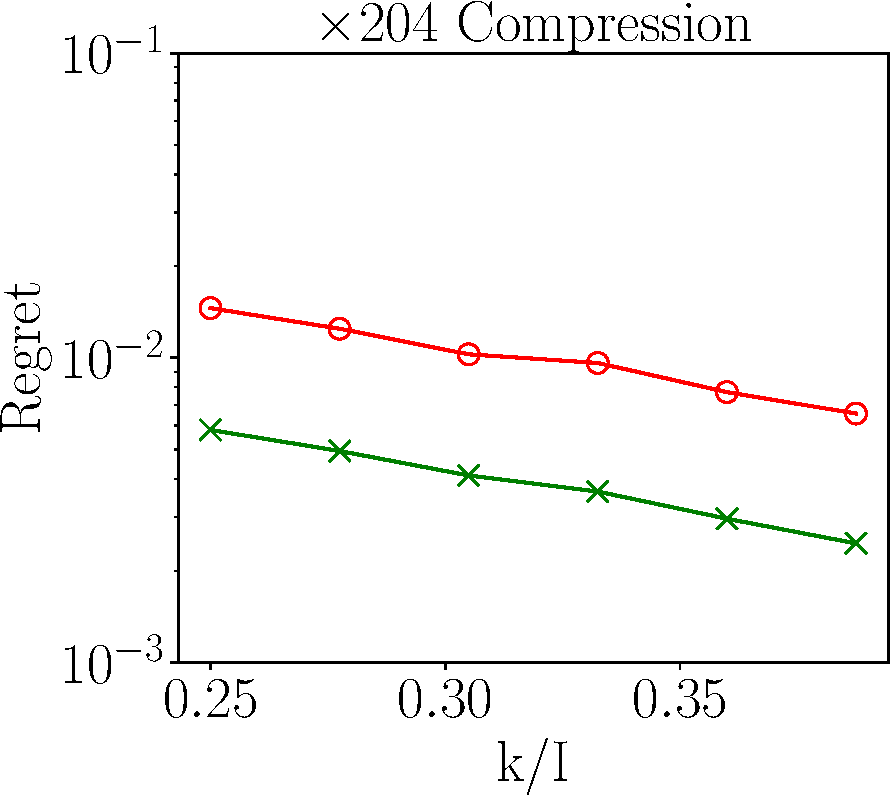
\includegraphics[height=2.9cm]{figure/multi_SRFRAD_frk8.pdf}
	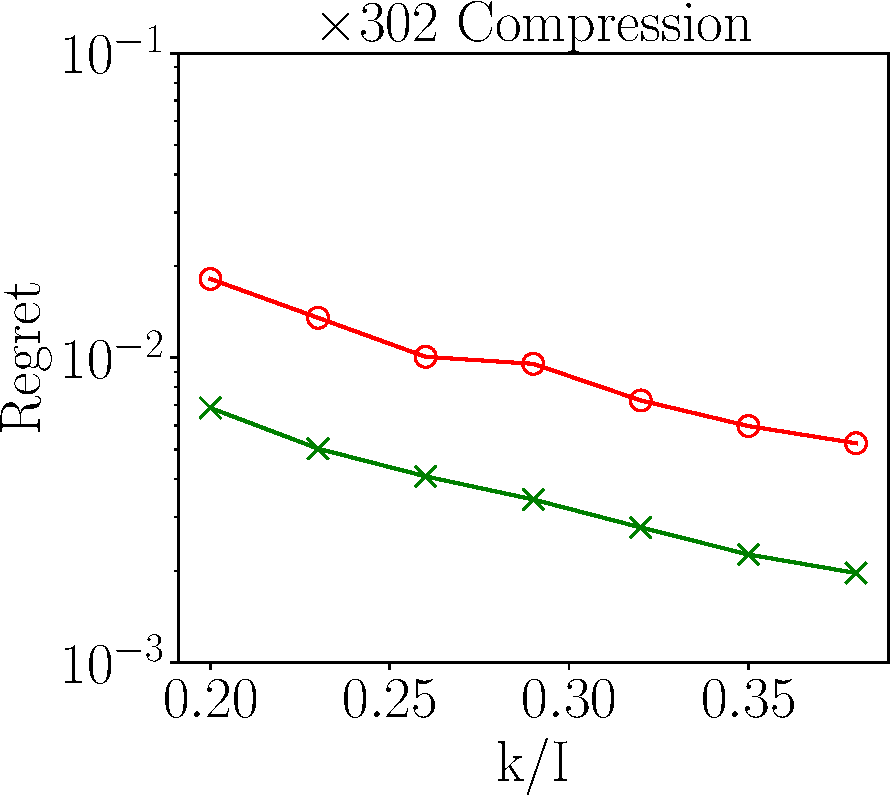
\includegraphics[height=2.9cm]{figure/multi_SRFRAD_frk10.pdf}
	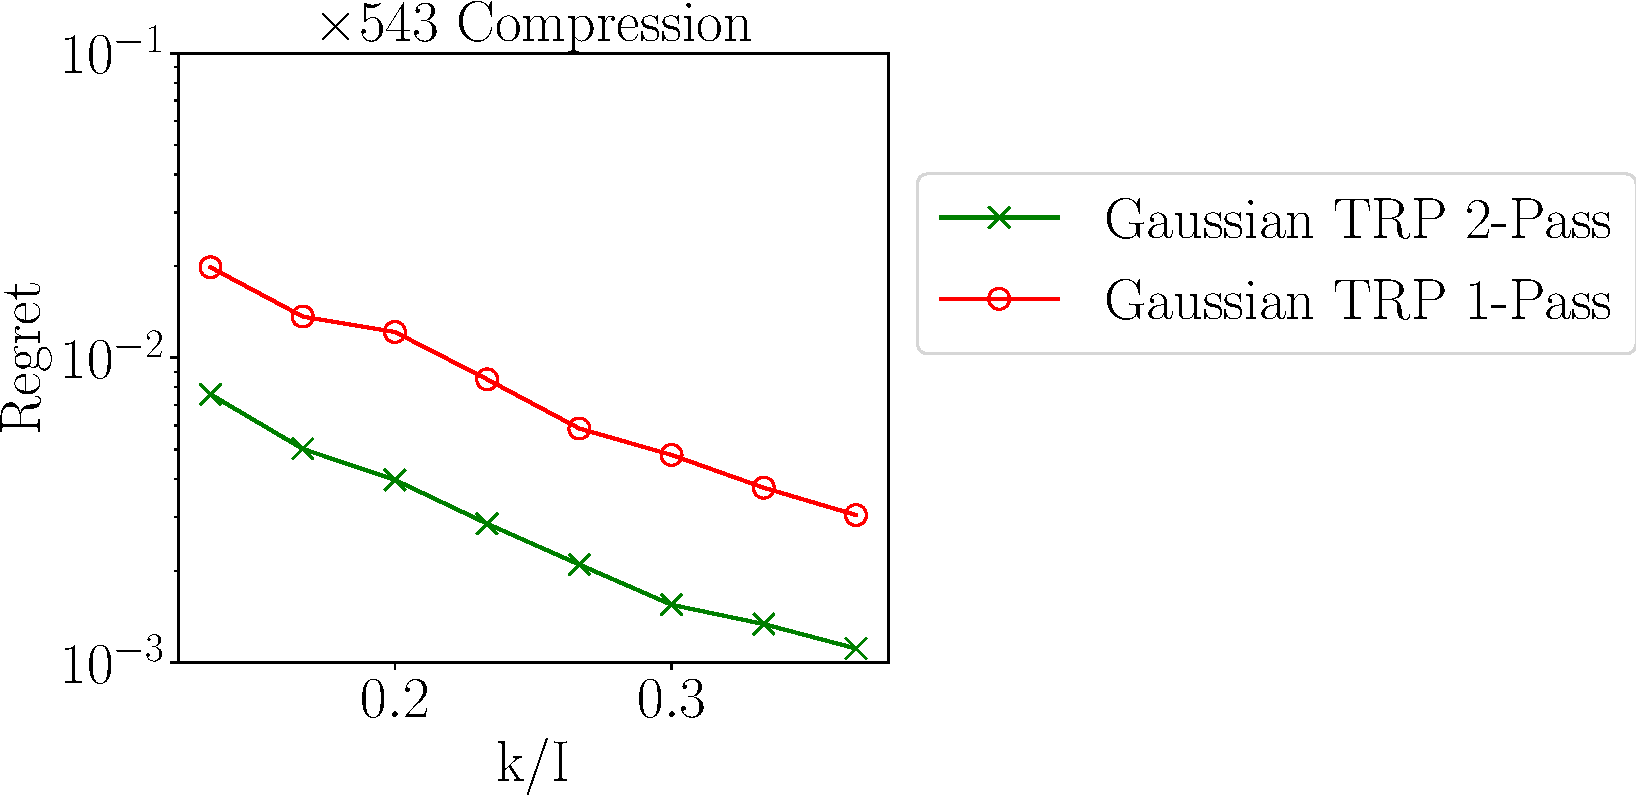
\includegraphics[height=2.9cm]{figure/multi_SRFRAD_frk15.pdf}\\
	\textbf{Net Radiative Flux at Surface}\\~\\
	\centering
	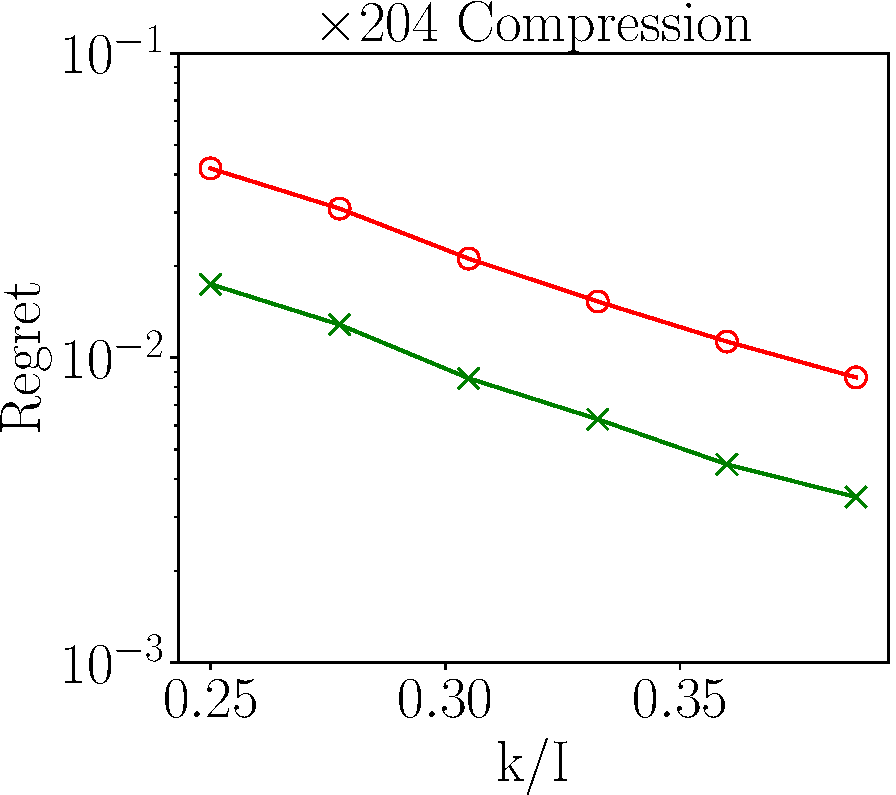
\includegraphics[height=2.9cm]{figure/multi_BURDENDUST_frk8.pdf}
	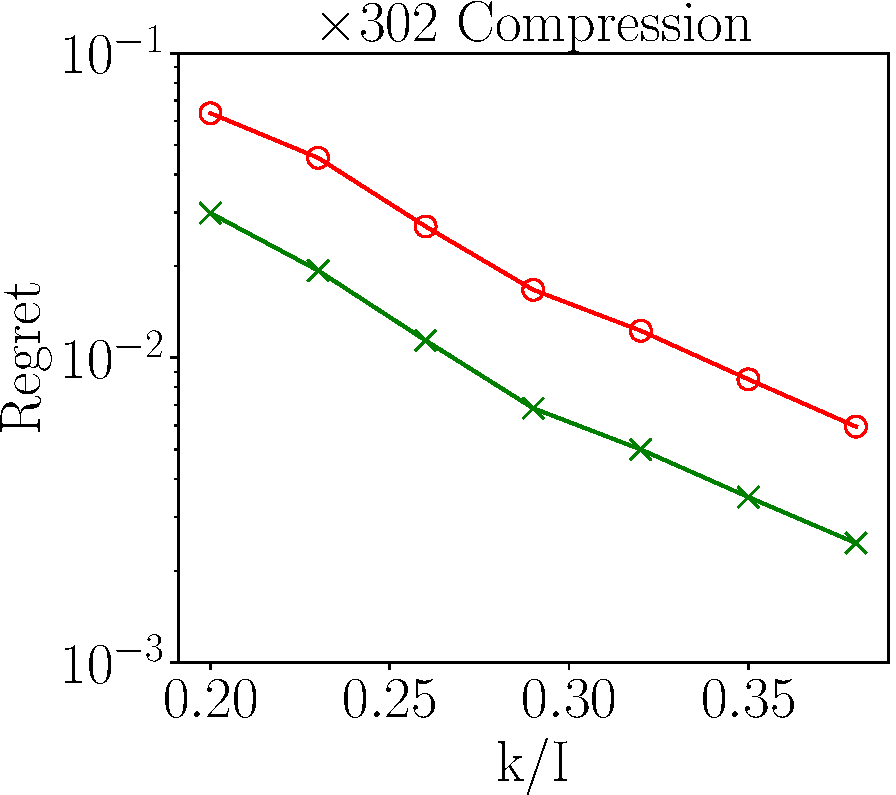
\includegraphics[height=2.9cm]{figure/multi_BURDENDUST_frk10.pdf}
	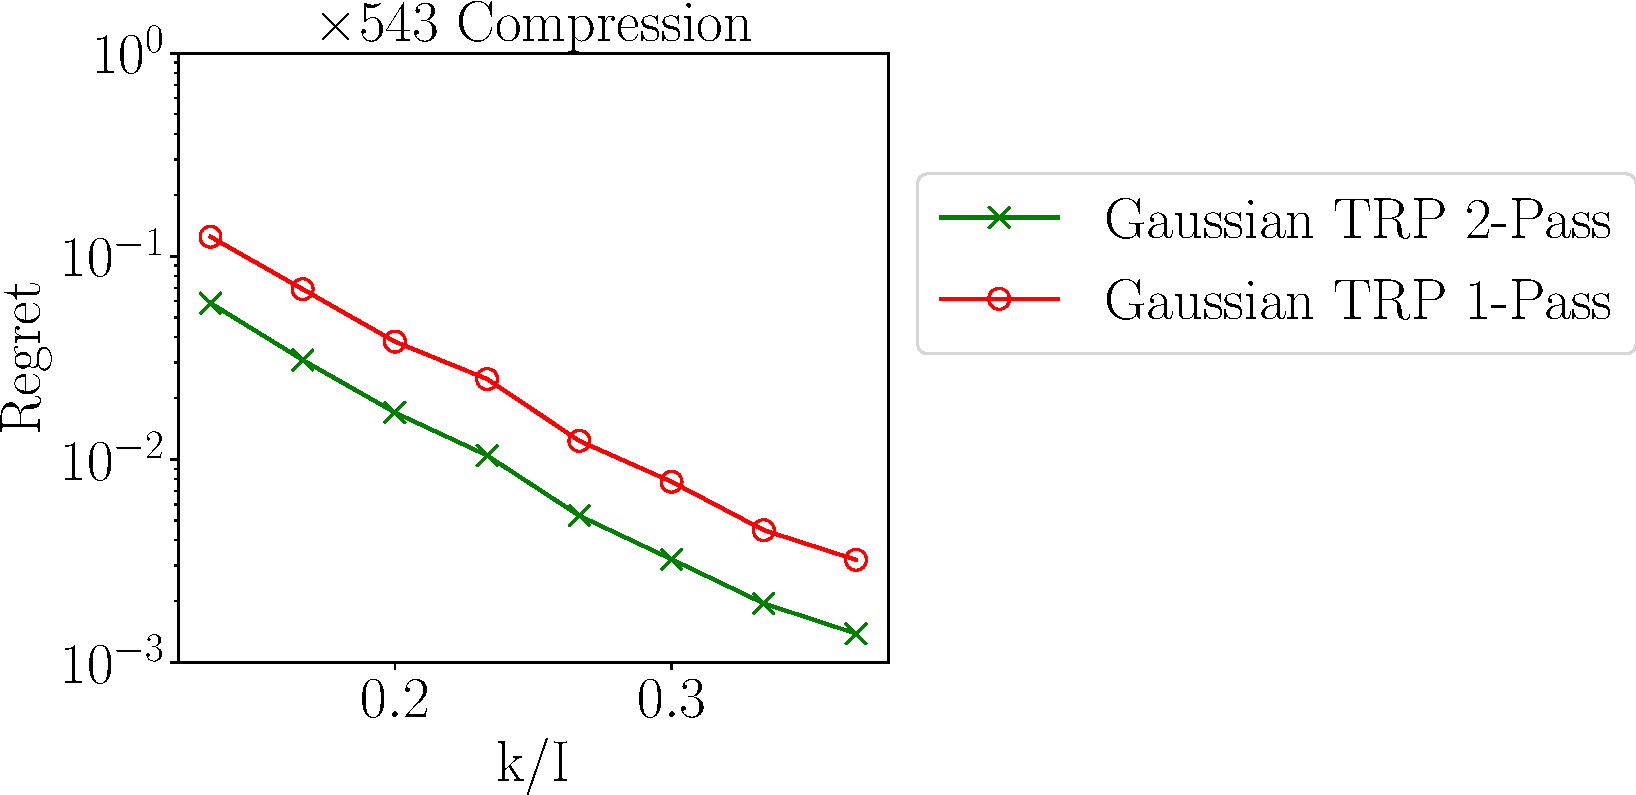
\includegraphics[height=2.9cm]{figure/multi_BURDENDUST_frk15.pdf}\\
	\textbf{Dust Aerosol Burden}
	\caption{We approximate the net radiative flux and dust aerosol burden data using our one-pass and two-pass algorithms using Gaussian TRP. We compare the performance under different ranks ($r/I = 0.125,0.2,0.067$). The dataset comes from the CESM CAM. The dust aerosol burden measures the amount of aerosol contributed by the dust. The net radiative flux determines the energy received by the earth surface through radiation. } \label{fig:srfrad_burden_dust}
\end{figure}
